\documentclass[titlepage]{article}
\usepackage[utf8]{inputenc}
\usepackage[margin=1in]{geometry}
\usepackage{graphicx}
\usepackage{enumitem}
\usepackage{placeins}
\usepackage{dirtree}
\usepackage{enumitem,amssymb}
\newlist{todolist}{itemize}{2}
\setlist[todolist]{label=$\square$}
\usepackage{multicol}
\usepackage{cprotect}
\usepackage{rotating}

\newlist{steps}{enumerate}{1}
\setlist[steps, 1]{label = Step \arabic*:}

\title{\Huge Groundhog Radar System Operation and Maintenance Manual}
\author{\LARGE Michael Christoffersen}
\date{\LARGE June 2024\\v1.1}

\begin{document}

\maketitle

\tableofcontents

\pagebreak

\section{Setup \& Operation}
\subsection{Setup}
\begin{enumerate}
    \item Lay out four antenna elements. Usually this is done in an endfire orientation that looks like this ( | | ) as opposed to a broadside orientation ( $\mid \hspace{1em} \mid$ ). A broadside orientation could cause significant coupling between the two antennas, leading to excess ringing.
    \item Set up the transmitter (pulser):
    \begin{enumerate}
        \item Connect the two tansmit antenna elements to the ``-ve'' and ``+ve'' ports.
        \item Connect a 12v battery to the ``DC power in'' ports.
        \item \textbf{Note}: Sometimes the pulser fails to begin pulsing when the power is connected so be sure to check that yellow ``Active'' light is on when the power is connected. If it is not you should disconnect the reconnect power.
        \item \textbf{Note}: It is best to connect the antenna elements before powering the transmitter to avoid a chance of a significant shock.
    \end{enumerate}
    
    \item Set up the receiver hardware \begin{enumerate}
        \item Connect the two antenna elements to the banana jacks on the receiver case.
        \item Wiring inside the receiver case:
        \begin{enumerate}
            \item Ensure that the first connection after the banana jacks is to the balun. The banana jacks should connect to the balanced side of the balun, which has a white ring on the BNC connector.
            \item Connect a low-pass filter after the balun. The frequency choice of the low-pass filter could depend on your antenna length, but should be no higher than 11 MHz. \textbf{Note}: This is likely not necessary and potentially harmful to data quality for glaciers less than 600m thick.
            \item If desisired, insert an amplifier after the low-pass filter and connect it to the power supply.
            \item The final part of the signal chain will be a BNC-SMA cable that connects to a RF limiter, which is connected to the \textbf{RF2} SMA port on the Ettus N210.
            \item Figure \ref{fig:wiring} shows a diagram of all of the connections inside of the receiver box.
        \end{enumerate}
        \item Ensure the USRP N210 (the radio) is powered. It should be supplied with 6v, either with a voltage regulator of some sort or a 6v battery.
        \item Connect the ethernet port of the USRP N210 to the ethernet port of the field laptop. 
        \item Connect the Ublox USB GNSS to a USB port of the field laptop.
        \item Connect a GNSS antenna to the Ublox USB GNSS SMA port.
        \item \textbf{Note}: Connecting USB devices other than the Ublox GNSS to the field laptop can potentially prevent communication with the GPS, so that should be avoided.
    \end{enumerate}

    \item Verify operation of the transmitter and receiver \begin{enumerate}
        \item When you boot up the field laptop it will open a terminal in the directory \\\verb+/home/radar/groundhog/control+.
        \begin{enumerate}
            \item If the laptop has not opened a terminal in this directory open a terminal, run \verb+source \~/.bashrc+, and then navigate to it.
        \end{enumerate}
        \item Configure the GNSS to output raw data and NMEA strings by running the script \verb+configure-gps.sh+.
        \item Run the GPS test script, \verb+./gps-test.sh+. after a 5 second delay it will print many NMEA sentences if the GNSS is communicating correctly with the field laptop and configured properly. If there are no GPGGA sentences printed see the GPS troubleshooting section of this document (\ref{trouble_gps}).
        \item Run the receiver test script, \verb+./plot_rx.py+. It will record and plot 5 milliseconds of samples. You should see several distinct spikes, the exact number will depend on the pulse repetition frequency of your transmitter. If no plot is generated see the USRP N210 troubleshooting section of this document (\ref{trouble_usrp}). If the plot appears to have only noise (no spikes) see the transmitter and antenna troubleshooting sections of this document (\ref{trouble_xmit}, \ref{trouble_ant}).
        \item Use the \verb+plot_rx.py+ plot to decide on a trigger threshold. The trigger works on absolute amplitude, so a positive or negative polarity signal with a larger amplitude than the trigger threshold will cause a trigger.
    \end{enumerate}

    \item Once you have verified operation of the transmitter and receiver you almost ready to acquire data (!). Change the trigger threshold in \verb+run_radar.sh+ to the value you chose from inspecting the plot generated by \verb+plot_rx.py+. You can use gedit, \verb+gedit run_radar.sh+, or your favorite terminal text editor. Make sure to save and close the file when you are finished. Now you are ready to acquire data.
\end{enumerate}

\begin{figure}[h]
\centering
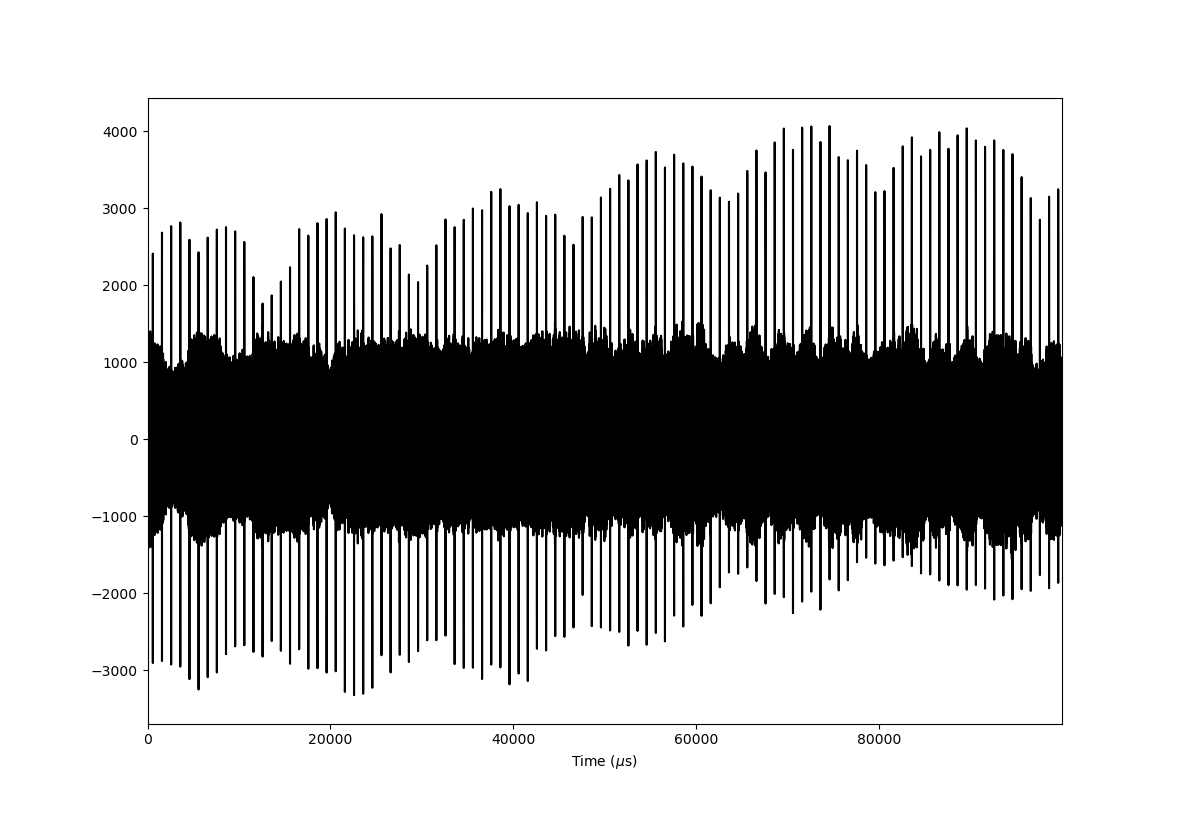
\includegraphics[width=\textwidth]{figs/plot_rx.png}
\cprotect\caption{An example of the graph produced by \verb:plotRX.py: when the transmitter and receiver are working properly. The positive and negative polarity amplitude spikes (to roughly +/- 3500 counts) are the transmitter pulses. The darker region of the plot is ambient noise and reflected pulses. This is from a particularly high ambient noise environment, which causes the apparent amplitude of the pulses to fluctuate.}
\label{fig:plot_rx}
\end{figure}

\subsection{Operation}
The \verb+run_radar.sh+ script operates the radar. It generates an unused filename, \verb|groundhogXXXX| (between \verb+groundhog0000+ and \verb+groundhog9999+) then starts two instances of \verb+gpspipe+, one which logs NMEA sentences to the file \verb|groundhogXXXX.txt| and another which logs all GNSS output (including raw data) to the file \verb|groundhogXXXX.ubx|. Then it starts the digitizer software which begins logging to \verb|groundhogXXXX.ghog|.

You'll run \verb|./run_radar| to begin data acquisition and then use \verb|Ctrl+c| to end it. The GPS and radar data files will be saved in the directory \verb|/home/radar/groundhog/data|.

\subsection{Processing}
The processing pipeline is small, all files are in \verb|/home/radar/groundhog/process|. The \verb|ghog2h5.py| script converts files from the groundhog digitizer format to HDF5. Running \verb|./ghog2h5.py --help| will print usage instructions.

The script \verb|makeQlook.py| generates quicklook images of the data inside each HDF5 file. Running \verb|./makeQlook.py --help| will print usage instructions.

There is a utility script in \verb|/home/radar/groundhog/control| named \verb|quicklook.sh| which will convert all files in \verb|/home/radar/groundhog/data| to HDF5 and generate quicklooks. It will then open the quicklooks which can be navigated with the arrow keys.

\section{Troubleshooting}
\subsection{GPS} \label{trouble_gps}
The GPS logging uses \verb|gpsd| to do the heavy lifting of communicating with the USB GPS. In \verb|run_radar.sh| the program \verb|gpspipe| is used to direct the real time output of the USB GPS to a file. If the GPS is not communicating with the computer for some reason the solution is likely a power cycle. The program \verb|gpsmon| can be run in the terminal to see the real-time output of the USB GPS. But when the GPS is configured properly (returning both NMEA sentences and raw data) \verb|gpsmon| will not show a proper fix because it is confused by the presence of the raw data and does not detect the NMEA strings. If there is no GPS information being received \verb|gpsmon| will show some JSON strings and nothing else.

\subsection{USRP N210} \label{trouble_usrp}
Need to flesh this out. Make sure that the ethernet connection is good. Make sure that the antennas are connected to the RF2 port. Make sure the power connector is properly seated - it is a bit undersized so can be finnicky sometimes.

\subsection{Kentech Pulser} \label{trouble_xmit}
There is not a lot that can go wrong with the Kentech pulser which will be user serviceable. If it is powered but not transmitting first try unplugging and re-plugging the power. If that fails check the fuse and see if it needs to be replaced.

\subsection{Antennas} \label{trouble_ant}
The resistively loaded antennas are probably the most moody part of this radar. It is difficult to make a strong mechanical connection between the two sides of wire that is also electrically insulating.

The most common antenna issue is a complete break or an intermittent connection at one of the resistors. This can be very difficult to locate, in the case of an intermitten connection the break is often only present when the antenna is under tension (being pulled).

There are a couple ways you can check an antenna. The quickest (if the antennas are laid out) is an antenna analyzer. This would qickly show if one of the elements has a break close to the feedpoint, as the antenna would be significantly de-tuned. The other method would be checking continuity with a multimeter. Use a pocket knife to strip some insulation from the antenna wire on either side of a resistor you want to check. Gently bending the antenna can help expose an intermittent connection.

\begin{sidewaysfigure}
\centering
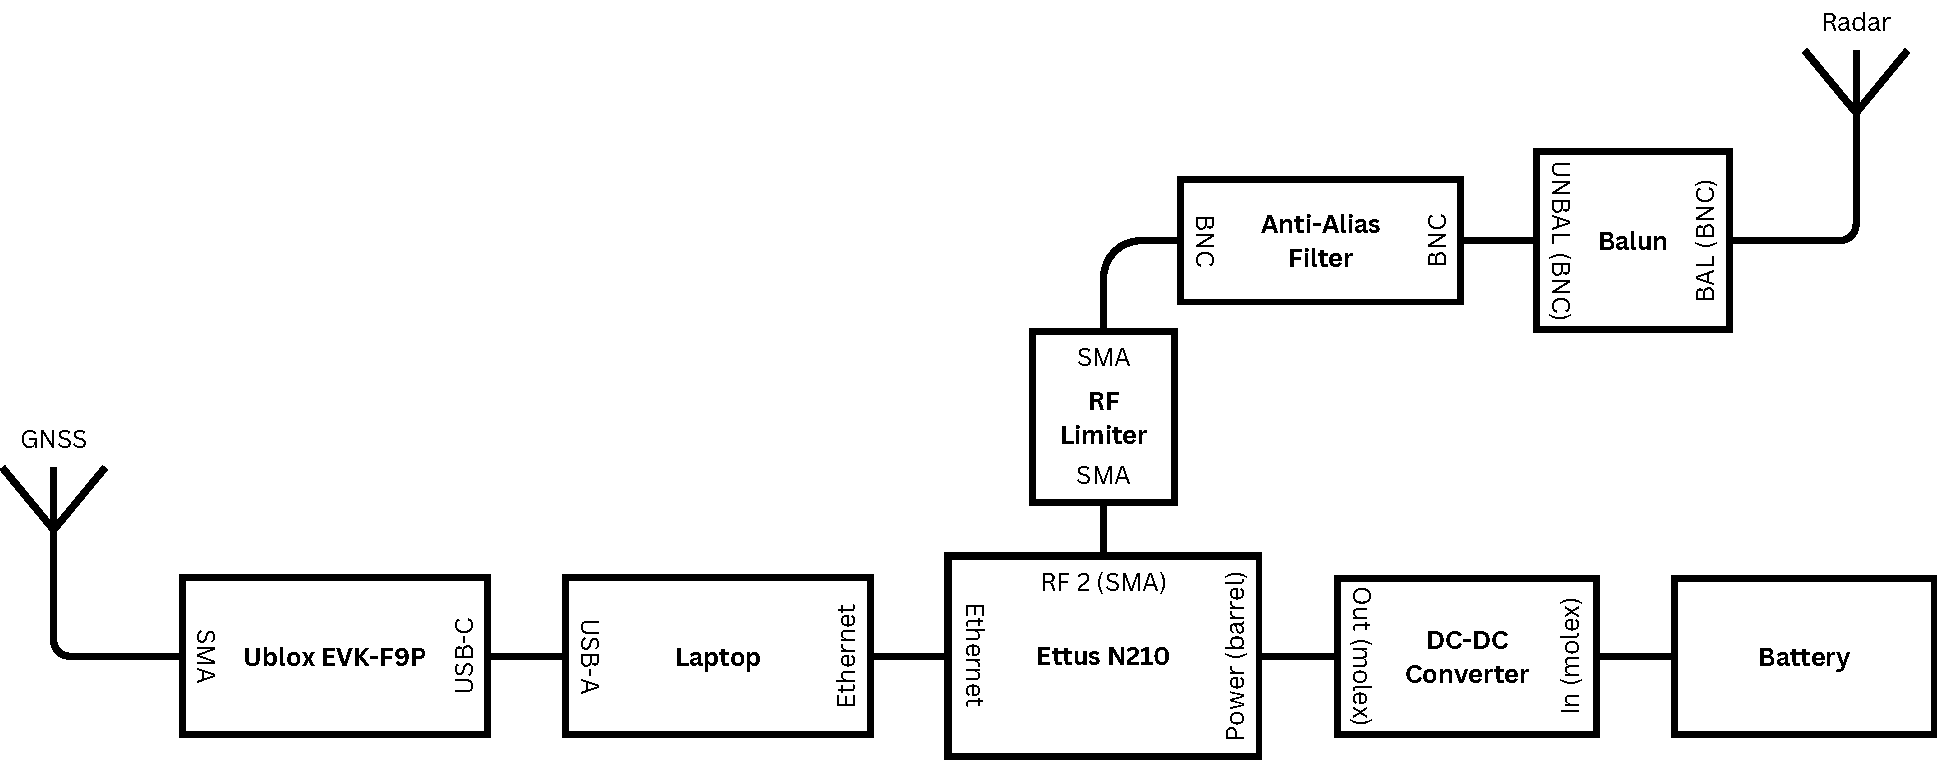
\includegraphics[width=\textwidth,height=\textheight,keepaspectratio]{figs/RadarWiringDiagram_noPPS.pdf}
\caption{Receiver box wiring diagram.}
\label{fig:wiring}
\end{sidewaysfigure}

\newpage
\section{Packing List}

\textbf{RX}
\begin{todolist}
    \item radio (N210)
    \item 2x antenna elements
    \item anti-alias filter
    \item preamplifier
    \item rf limiter
    \item rugged laptop
    \item rx battery
    \item rx pelican case
    \item balun
    \item cables?
\end{todolist}
\textbf{TX}
\begin{todolist}
   \item kentech pulser
    \item spare fuses and capacitors for kentech
    \item 2x antenna elements
    \item tx battery
    \item tx pelican case
    \item cables?
\end{todolist}
\textbf{Misc}
\begin{todolist}
    \item sleds
    \item rope
    \item spare resistors for antennas
    \item spare heat shrink tubing
    \item heat gun
    \item soldering iron
    \item solder
    \item flux
    \item antenna analyzer
    \item spare wire
    \item spare ring/spade terminals
    \item other spares?
\end{todolist}

\end{document}
